\section{Results}
\fred (v0.0.3)\cite{stephen_thompson_2020_3946090} was used at our Medical Summer School in 2020 with a cohort of 5 students. Feedback suggested that it had improved their understanding
of fiducial based registration. The results of the game based usability study are shown in Figure \ref{fig:usability}. As expected scores are 
highest when the actual \gls{TRE} is known. Interestingly it appears that when told only the expected value of the \gls{FLE} the students
tended to under treat the target more, resulting in lower overall scores. This study currently only has 100 data points (20 for each category)
so it must be stated that the results are not yet statistically significant. 

\begin{figure}
        \begin{center}
        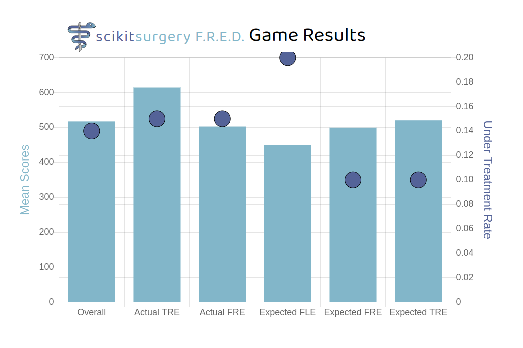
\includegraphics[width=0.7\linewidth]{usability.eps}
                \caption{\label{fig:usability}Average scores and treatment failure rates for the game based usability study.}
	\end{center}
\end{figure}


